\documentclass[%
    a4paper,
    oneside,
    punct=kaiming,
    zihao=-4,
    landscape
]{ctexbook}

\providecommand*{\laauxtoro}{the \textsf{mwe}
    (Minimal Working Example) package}
\providecommand*{\lailustrajxo}{\includepdf{example-image-a4-landscape.pdf}}

\usepackage[margin=2.5cm]{geometry}
\pagestyle{empty}

\IfFontExistsTF{FiraSans-Regular.otf}{%
    \IfFontExistsTF{FiraSans-SemiBold.otf}{%
        \IfFontExistsTF{FiraSans-Italic.otf}{%
            \IfFontExistsTF{FiraSans-SemiBoldItalic.otf}{%
                \setmainfont{FiraSans}[
                    Path,
                    UprightFont = *-Regular.otf,
                    BoldFont = *-SemiBold.otf,
                    ItalicFont = *-Italic.otf,
                    BoldItalicFont = *-SemiBoldItalic.otf
                ]
                \setsansfont{FiraSans}[
                    Path,
                    UprightFont = *-Regular.otf,
                    BoldFont = *-SemiBold.otf,
                    ItalicFont = *-Italic.otf,
                    BoldItalicFont = *-SemiBoldItalic.otf
                ]
            }{}
        }{}
    }{}
}{}

\IfFontExistsTF{Sarasa Mono SC}{%
    \IfFontExistsTF{Sarasa Mono SC Italic}{%
        \IfFontExistsTF{Sarasa Mono SC SemiBold}{%
            \IfFontExistsTF{Sarasa Mono SC SemiBold Italic}{%
                \PassOptionsToClass{fontset=none}{ctexbook}
                \setmonofont{Sarasa Mono SC}[
                    UprightFont = *,
                    BoldFont = * SemiBold,
                    ItalicFont = * Italic,
                    BoldItalicFont = * SemiBold Italic
                ]
                \setCJKmainfont{Sarasa Mono SC}[
                    UprightFont = *,
                    BoldFont = * SemiBold,
                    ItalicFont = * Italic,
                    BoldItalicFont = * SemiBold Italic
                ]
                \setCJKsansfont{Sarasa Mono SC}[
                    UprightFont = *,
                    BoldFont = * SemiBold,
                    ItalicFont = * Italic,
                    BoldItalicFont = * SemiBold Italic
                ]
                \setCJKmonofont{Sarasa Mono SC}[
                    UprightFont = *,
                    BoldFont = * SemiBold,
                    ItalicFont = * Italic,
                    BoldItalicFont = * SemiBold Italic
                ]
            }{}
        }{}
    }{}
}{
    \IfFontExistsTF{SarasaMonoSC-Regular.ttf}{%
        \IfFontExistsTF{SarasaMonoSC-Italic.ttf}{%
            \IfFontExistsTF{SarasaMonoSC-SemiBold.ttf}{%
                \IfFontExistsTF{SarasaMonoSC-SemiBoldItalic.ttf}{%
                    \PassOptionsToClass{fontset=none}{ctexbook}
                    \setmonofont{SarasaMonoSC}[
                        Path,
                        UprightFont = *-Regular.ttf,
                        BoldFont = *-SemiBold.ttf,
                        ItalicFont = *-Italic.ttf,
                        BoldItalicFont = *-SemiBoldItalic.ttf
                    ]
                    \setCJKmainfont{SarasaMonoSC}[
                        Path,
                        UprightFont = *-Regular.ttf,
                        BoldFont = *-SemiBold.ttf,
                        ItalicFont = *-Italic.ttf,
                        BoldItalicFont = *-SemiBoldItalic.ttf
                    ]
                    \setCJKsansfont{SarasaMonoSC}[
                        Path,
                        UprightFont = *-Regular.ttf,
                        BoldFont = *-SemiBold.ttf,
                        ItalicFont = *-Italic.ttf,
                        BoldItalicFont = *-SemiBoldItalic.ttf
                    ]
                    \setCJKmonofont{SarasaMonoSC}[
                        Path,
                        UprightFont = *-Regular.ttf,
                        BoldFont = *-SemiBold.ttf,
                        ItalicFont = *-Italic.ttf,
                        BoldItalicFont = *-SemiBoldItalic.ttf
                    ]
                }{}
            }{}
        }{}
    }{}
}

\usepackage[
    math-style=ISO,
    bold-style=ISO,
    mathrm=sym,
    mathbf=sym,
]{unicode-math}
\IfFontExistsTF{FiraMath-Regular.otf}{%
    \setmathfont{FiraMath-Regular.otf}
}{}

\makeatletter
\providecommand*{\midsloppy}{%
    \tolerance 5000%
    \hbadness 4000%
    \emergencystretch 1.5em%
    \hfuzz .1\p@%
    \vfuzz\hfuzz}
\makeatother

\renewcommand*{\familydefault}{\sfdefault}

\AtBeginDocument{%
    \frenchspacing
    \midsloppy
    \renewcommand*{\UrlFont}{\ttfamily}
}

\usepackage[breaklinks,hidelinks,unicode]{hyperref}
\usepackage{xurl}

\usepackage{caption}
\usepackage{subcaption}
\usepackage{pdfpages}

\begin{document}

\lailustrajxo
\clearpage

\noindent\phantom{\parbox{\linewidth}{\footnotesize%
        \texttt{©} Determinantulo.
        All rights reserved.\\
        The illustration on the reverse side was drawn by
        \laauxtoro.%
    }}

\vfill

\begin{align*}
    \det \begin{bmatrix}
             a_{1,1} & a_{1,2} & a_{1,3} \\
             a_{2,1} & a_{2,2} & a_{2,3} \\
             a_{3,1} & a_{3,2} & a_{3,3} \\
         \end{bmatrix}
    =
    a_{1,1} a_{2,2} a_{3,3}
    + a_{1,2} a_{2,3} a_{3,1}
    + a_{1,3} a_{2,1} a_{3,2}
    - a_{1,1} a_{2,3} a_{3,2}
    - a_{1,2} a_{2,1} a_{3,3}
    - a_{1,3} a_{2,2} a_{3,1}
\end{align*}

\begin{figure*}[h!]
    \centering
    \begin{minipage}[h!]{0.49\textwidth}
        \centering
        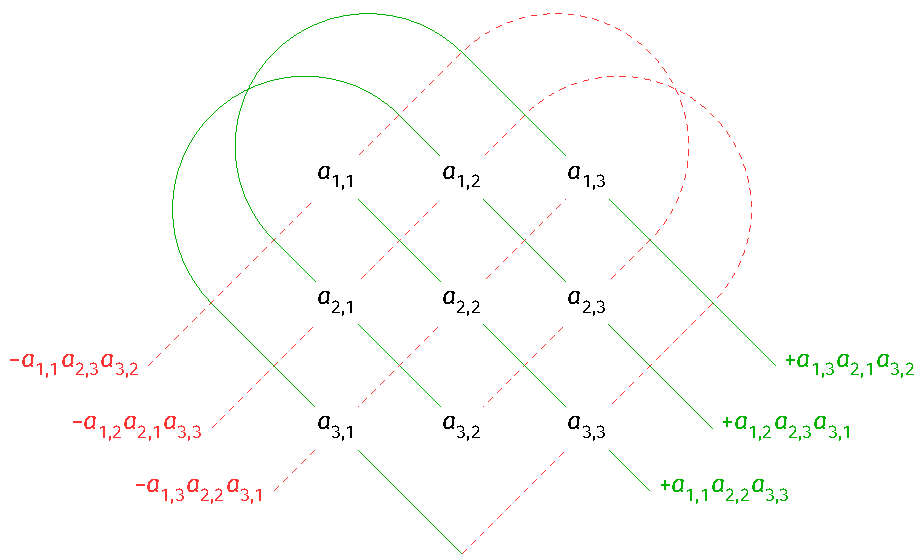
\includegraphics[width=\textwidth]{koro}

        \caption*{%
            \centering%
            Memorhelpilo de la determinanto de \(3 \times 3\)-matrico\\
            A mnemonic device of the determinant of a \(3 \times 3\) matrix\\
            \(3 \times 3\) 阵的行列式的记忆方法}
    \end{minipage}
    \hfill
    \begin{minipage}[h!]{0.49\textwidth}
        \centering
        \begin{subfigure}{\textwidth}
            \centering
            
\includegraphics{rapidresponda kodo por GitHub}
            \caption*{\url{https://github.com/septsea/det}}
        \end{subfigure}

        \,

        \begin{subfigure}{\textwidth}
            \centering
            
\includegraphics{rapidresponda kodo por Gitee}
            \caption*{\url{https://gitee.com/septsea/det}}
        \end{subfigure}

        % \vspace{1ex}

        \caption*{%
            \centering%
            Legu \textit{Enkonduko al determinantoj} por pli multaj informoj.\\
            Read \textit{An introduction to determinants} for more information.\\
            阅读\,《行列式入门》\,以了解更多.}
    \end{minipage}
\end{figure*}

\vfill

\noindent\parbox{\linewidth}{\footnotesize%
    \texttt{©} Determinantulo.
    All rights reserved.\\
    The illustration on the reverse side was drawn by
    \laauxtoro.%
}

\end{document}
